\documentclass[tikz,border=4pt]{standalone}
\usepackage{ctex}
\usepackage{amsmath}
\usetikzlibrary{arrows.meta}

% p8-05a: 图象法解方程组——两直线交点 = 方程组的解
% 方程组: y=2x-1, y=-x+5, 交点(2,3)
\begin{document}
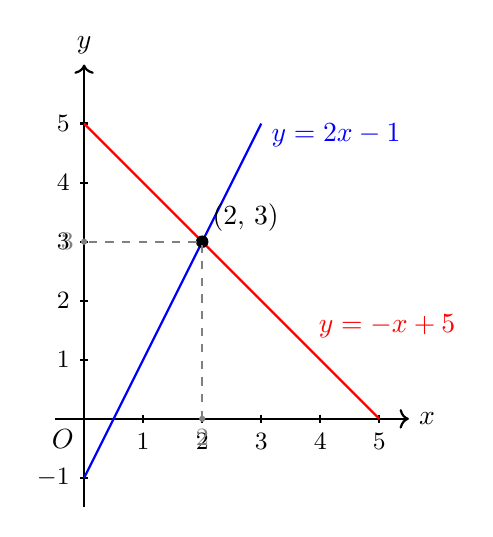
\begin{tikzpicture}[scale=0.75, thick]
  % 坐标轴
  \draw[->] (-0.5,0) -- (5.5,0) node[right] {$x$};
  \draw[->] (0,-1.5) -- (0,6.0) node[above] {$y$};
  \node[below left] at (0,0) {$O$};

  % 刻度
  \foreach \x in {1,2,3,4,5} {
    \draw (\x, 2pt) -- (\x, -2pt) node[below] {\small$\x$};
  }
  \foreach \y in {-1,1,2,3,4,5} {
    \draw (2pt,\y) -- (-2pt,\y) node[left] {\small$\y$};
  }

  % 直线 y = 2x-1（经过(0,-1)和(1,1)）
  \draw[blue, thick] (0,-1) -- (3.0, 5.0);
  \node[right, blue] at (3.0, 4.8) {$y=2x-1$};

  % 直线 y = -x+5（经过(0,5)和(5,0)）
  \draw[red, thick] (0,5) -- (5, 0);
  \node[above right, red] at (3.8, 1.2) {$y=-x+5$};

  % 交点 (2,3)
  \fill (2,3) circle (3pt);
  \node[above right] at (2,3) {$(2,\,3)$};

  % 辅助虚线
  \draw[gray, dashed] (2,0) -- (2,3) -- (0,3);
  \fill[gray] (2,0) circle (1.5pt) node[below] {\small$2$};
  \fill[gray] (0,3) circle (1.5pt) node[left] {\small$3$};
\end{tikzpicture}
\end{document}
